\subsubsection{Lambda}\label{Lambda}

Lambda is part of hybrid architecture, that means it combines batch and real time processing. Since both processes are used, it is common to split them apart. We would have batch processing for bigger files and real time (or speed) for time intense applications \parencite{lin2017lambda}.

One real world example would be airline customers. We can split them into priority and none priority. Both achieve the same goal, just one type of customers will be served first.

In our example, we could use Lambda architecture. For example, game data (how players are moving) needs to be processed in real time. But chat data can be processed as a batch. Reason for this is chat data doesn't provide as much value to us as game data.

\begin{figure}[H]
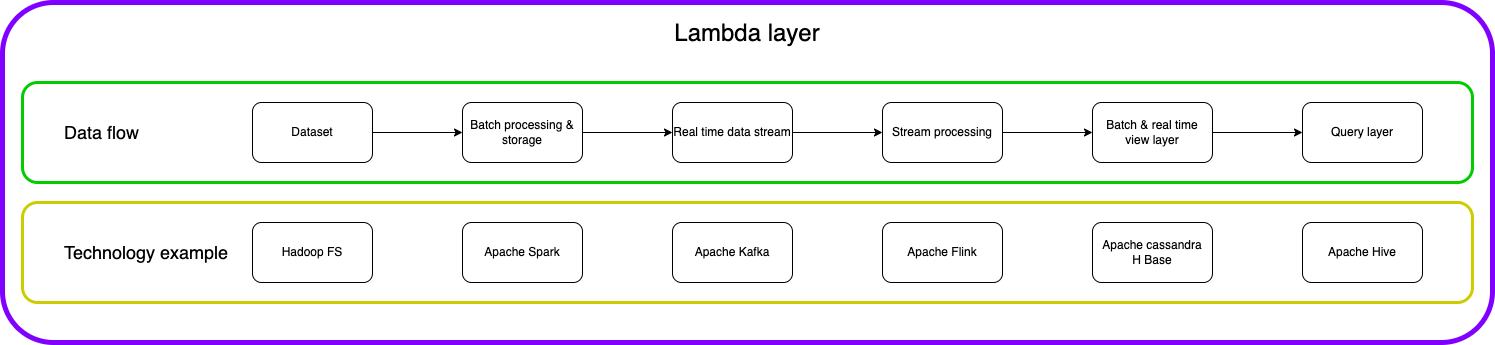
\includegraphics[scale=0.25]{img/ProcessingParadigms/BigData-Lambda.png}
\centering
\caption{Lambda}
\label{fig:Lambda}
\end{figure}